% ============================================================
%  Chapter 3: Generating Random Variables
%  Lectures on Monte Carlo Theory --- Leskel\"a & Vihola
% ============================================================
\documentclass[aspectratio=169,10pt]{beamer}

\usetheme{Madrid}
\usecolortheme{seahorse}

\usepackage[utf8]{inputenc}
\usepackage[T1]{fontenc}
\usepackage{amsmath,amssymb,amsthm}
\usepackage{mathtools}
\usepackage{bm}
\usepackage{graphicx}
\usepackage{booktabs}
\usepackage{listings}
\usepackage{xcolor}
\usepackage{multicol}
\usepackage{tikz}

\graphicspath{{figures/}}

\lstdefinestyle{python}{
  language=Python,
  basicstyle=\ttfamily\scriptsize,
  numbers=left,
  numberstyle=\tiny\color{gray},
  frame=single,
  backgroundcolor=\color{gray!7},
  keywordstyle=\color{blue!70!black}\bfseries,
  commentstyle=\color{green!50!black}\itshape,
  stringstyle=\color{red!60!black},
  showstringspaces=false,
  breaklines=true,
  xleftmargin=1.5em,
  framexleftmargin=1.5em,
}

\setbeamertemplate{footline}[frame number]
\setbeamertemplate{navigation symbols}{}

% -- shorthand macros ------------------------------------------
\newcommand{\PP}{\mathbb{P}}
\newcommand{\EE}{\mathbb{E}}
\newcommand{\RR}{\mathbb{R}}
\newcommand{\UU}{\mathcal{U}}
\newcommand{\NN}{\mathcal{N}}
\newcommand{\FInv}{F^{\leftarrow}}
\DeclareMathOperator{\Vol}{Vol}

% ============================================================
\title[Ch.\,3: Generating Random Variables]{%
  Chapter 3: Generating Random Variables}
\subtitle{Lectures on Monte Carlo Theory --- Leskel\"a \& Vihola}
\author{}
\date{}
% ============================================================

\begin{document}

\begin{frame}
  \titlepage
\end{frame}

% -- Table of Contents ------------------------------------------
\begin{frame}{Chapter Overview}
  \begin{columns}[t]
    \column{0.5\textwidth}
    \tableofcontents[sections={1-5}]
    \column{0.5\textwidth}
    \tableofcontents[sections={6-12}]
  \end{columns}
\end{frame}

\AtBeginSection[]{
  \begin{frame}{Outline}
    \tableofcontents[currentsection, hideallsubsections]
  \end{frame}
}

% ============================================================
\section{3.1 Inverse Transform Method (ITM)}
% ============================================================

\begin{frame}{3.1 Inverse Transform Method --- Motivation}
  \textbf{Goal:} Generate $X$ with a given c.d.f.\ $F(x)=\PP(X\le x)$.

  \medskip
  \textbf{Key idea:} If we can \emph{invert} $F$, we can transform a
  $\UU[0,1)$ sample into a sample from $F$.

  \medskip
  \begin{block}{Generalized Inverse (Quantile Function)}
    \[
      \FInv(u) = \inf\{x : u \le F(x)\}, \qquad u\in(0,1).
    \]
    \begin{itemize}
      \item $\FInv(u)$ is the \emph{generalized inverse} (or quantile function) of $F$.
      \item If $F$ is strictly increasing and continuous, $\FInv = F^{-1}$.
      \item $\FInv$ is non-decreasing and left-continuous.
    \end{itemize}
  \end{block}

  \medskip
  \textbf{Tail:} Define $\overline{F}(x)=1-F(x)$.  Then
  $\overline{F}^{\leftarrow}(u)=\FInv(1-u)$.
\end{frame}

\begin{frame}{Properties of the Generalized Inverse}
  \begin{block}{Key Properties}
    \begin{enumerate}[(P1)]
      \item $\FInv(u)$ is non-decreasing, left-continuous, with a right limit at $u$.
      \item If $F$ is strictly increasing and $u\in F(\RR)$: $u=F(x)$ iff $\FInv(u)=x$.
      \item $\FInv(F(x))\le x$; if $F$ is strictly increasing, $\FInv(F(x))=x$.
      \item $F(F^{\leftarrow}(u))\ge u$; equality holds when $F$ is continuous.
    \end{enumerate}
  \end{block}

  \begin{block}{Lemma 3.1.1 --- Fundamental Equivalence}
    \[
      u \le F(x) \iff \FInv(u) \le x.
    \]
    Consequently, if $F$ is continuous, $F(\FInv(u))=u$.
  \end{block}

  \begin{figure}
    \centering
    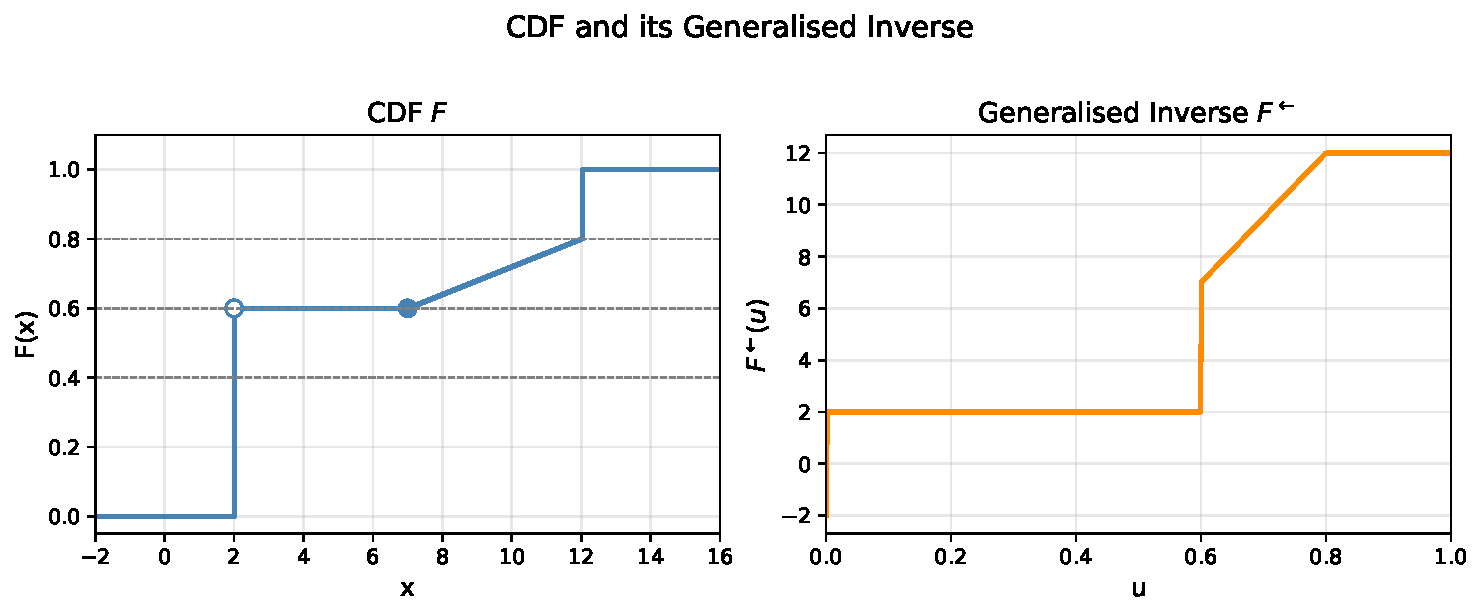
\includegraphics[width=0.72\textwidth]{fig_generalized_inverse}
    \caption{CDF $F$ (left) and its generalized inverse $\FInv$ (right).
      Note the flat region in $F$ creates a jump in $\FInv$, and
      a jump in $F$ creates a flat region in $\FInv$.}
  \end{figure}
\end{frame}

\begin{frame}{The ITM Theorem and Algorithm}
  \begin{block}{Proposition 3.1.2 --- The ITM Theorem}
    \begin{enumerate}[(a)]
      \item If $U\sim\UU[0,1)$, then $\FInv(U)\sim F$.
      \item If $F$ is continuous and $X\sim F$, then $F(X)\sim\UU[0,1)$.
    \end{enumerate}
  \end{block}

  \medskip
  \textbf{Proof sketch:}
  \[
    \PP(\FInv(U)\le x) = \PP(U\le F(x)) = F(x).
  \]

  \bigskip
  \begin{alertblock}{Algorithm 6 --- ITM}
    \textbf{Require:} c.d.f.\ $F$. \quad \textbf{Ensure:} $X\sim F$.
    \begin{enumerate}
      \item Generate $U\sim\UU[0,1)$.
      \item Set $X = \FInv(U)$.
      \item \textbf{return} $X$.
    \end{enumerate}
  \end{alertblock}

  \medskip
  \textbf{Corollary 3.1.3:} If $F$ is continuous, the $p$-value $p=F(T)$ is uniform on $[0,1)$.
\end{frame}

\begin{frame}[fragile]{3.1 Example: Exponential Distribution}
  \begin{columns}
    \column{0.48\textwidth}
    \begin{block}{Exponential Distribution $\mathrm{Exp}(\lambda)$}
      \[
        F(x) = \begin{cases} 0 & x < 0 \\ 1 - e^{-\lambda x} & x \ge 0 \end{cases}
      \]
      Mean $= 1/\lambda$, Variance $= 1/\lambda^2$.

      \medskip
      Generalized inverse of $\overline{F}$:
      \[
        \overline{F}^{\leftarrow}(u) = -\frac{1}{\lambda}\log(u).
      \]
    \end{block}

    \textbf{Algorithm 7 (ITM-Exp):}
    \begin{enumerate}
      \item $U\sim\UU[0,1)$
      \item $X = -\log(U)/\lambda$
      \item \textbf{return} $X$
    \end{enumerate}

    \column{0.50\textwidth}
    \begin{lstlisting}[style=python, caption={ITM for Exponential}]
import numpy as np
rng = np.random.default_rng(42)

def sample_exp(lam, n, rng):
    """Generate n samples ~ Exp(lam) via ITM."""
    U = rng.uniform(0, 1, n)
    return -np.log(U) / lam

X = sample_exp(lam=2.0, n=5000, rng=rng)
print(f"Mean: {X.mean():.4f} (theory: {0.5:.4f})")
print(f"Var:  {X.var():.4f}  (theory: {0.25:.4f})")
    \end{lstlisting}

    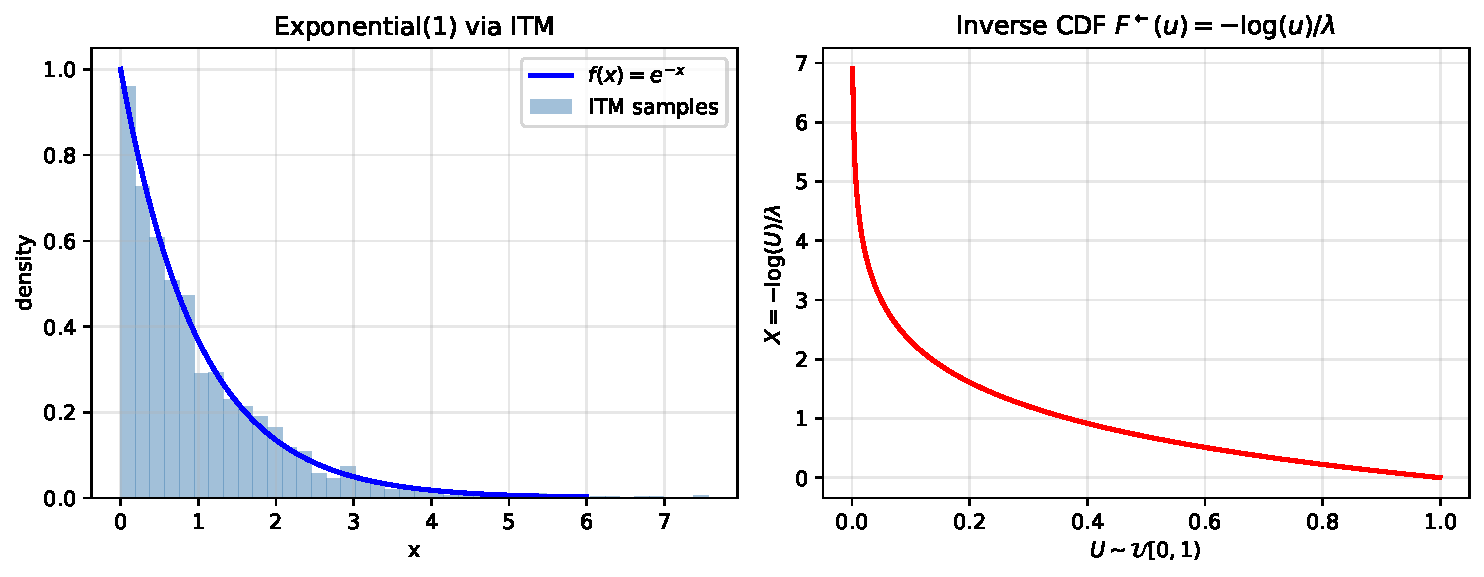
\includegraphics[width=\textwidth]{fig_itm_exponential}
  \end{columns}
\end{frame}

\begin{frame}{3.1 Pareto Distribution (Heavy Tail)}
  \begin{columns}
    \column{0.52\textwidth}
    \begin{block}{Pareto Distribution $\mathrm{Par}(\alpha)$}
      \[
        F(x) = \begin{cases} 0 & x < 0 \\ 1 - \dfrac{1}{(1+x)^\alpha} & x \ge 0 \end{cases}
      \]
      \begin{itemize}
        \item $\alpha$ --- shape parameter (tail index)
        \item $\EE X = \frac{1}{\alpha-1}$ (if $\alpha > 1$)
        \item Heavy-tailed: $\EE e^{sX} = \infty$ for all $s>0$
      \end{itemize}

      \medskip
      ITM: $\overline{F}^{\leftarrow}(u) = u^{-1/\alpha} - 1$

      \textbf{Algorithm 8 (ITM-Par):}
      \begin{enumerate}
        \item $U\sim\UU[0,1)$
        \item $X = U^{-1/\alpha} - 1$
        \item \textbf{return} $X$
      \end{enumerate}
    \end{block}

    \column{0.46\textwidth}
    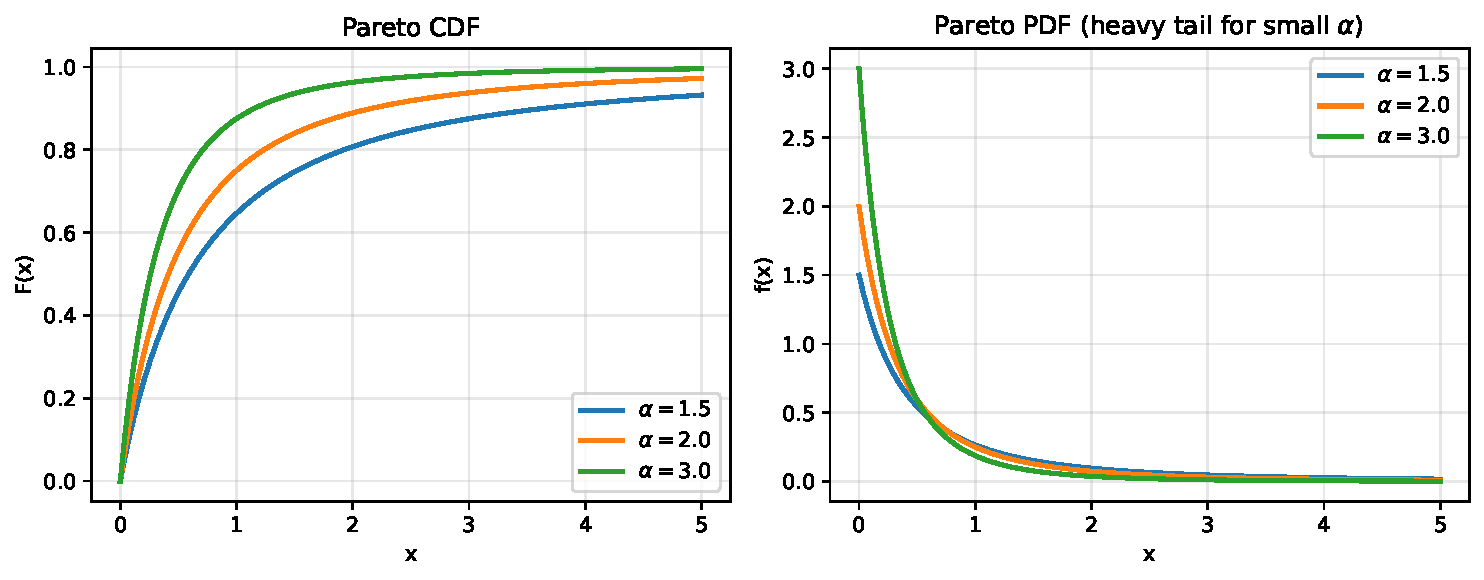
\includegraphics[width=\textwidth]{fig_pareto}
    \vspace{0.5em}
    \footnotesize
    Pareto CDF (top) and PDF (bottom) for $\alpha=1.5, 2, 3$.
    Smaller $\alpha$ $\Rightarrow$ heavier tail.
  \end{columns}
\end{frame}

% ============================================================
\section{3.2 ITM for Lattice Distributions}
% ============================================================

\begin{frame}[allowframebreaks]{3.2 ITM Variants for Lattice Distributions}
  \textbf{Setting:} $X$ takes values in $\{0,1,2,\ldots\}$ with probability function
  $(p_k)$, $k=0,1,\ldots$

  \begin{block}{Proposition 3.2.1 --- Discrete ITM}
    Let $U\sim\UU[0,1)$.  The random variable
    \[
      Y = \min\!\left\{k : U \le \sum_{i=0}^{k} p_i\right\}
    \]
    has probability function $(p_k)$.
  \end{block}

  \textbf{Algorithm 9 (ITM-d):}  sequentially add probabilities until cumulative sum $\ge U$.
  Expected number of loop iterations = $\EE Y + 1$.

  \framebreak

  \textbf{Efficient variant (Algorithm 10, ITR):} When the ratio
  $c_{k+1} = p_{k+1}/p_k$ is easily computable (e.g., Binomial, Poisson,
  Negative Binomial), use the recursion directly --- avoids storing the full PMF.

  \begin{block}{The $(a,b,0)$ class of distributions}
    A PMF satisfies $p_k = p_{k-1}(a + b/k)$ for $k=1,2,\ldots$
    \begin{itemize}
      \item \textbf{Binomial B}$(n,p)$: $c_{k+1} = \dfrac{p(n-k)}{(1-p)(k+1)}$
      \item \textbf{Poisson Poi}$(\lambda)$: $c_{k+1} = \dfrac{\lambda}{k+1}$
      \item \textbf{Neg.\ Binomial NB}$(r,p)$: $c_{k+1} = \dfrac{(r+k)p}{k+1}$
    \end{itemize}
  \end{block}

  \framebreak

  \begin{block}{Geometric Distribution $\mathrm{Geo}(p)$}
    PMF: $p_k = (1-p)p^k$, $k=0,1,\ldots$

    \medskip
    Mean $= p/q$ where $q=1-p$.

    \medskip
    \textbf{Closed-form ITM:}
    \[
      X = \lfloor \log U / \log p \rfloor \sim \mathrm{Geo}(p).
    \]
    \textit{Proof:}
    \[
      \PP(X \ge k) = \PP(\lfloor \log U / \log p\rfloor \ge k)
                  = \PP(\log U \le k\log p) = \PP(U \le p^k) = p^k.
    \]
  \end{block}

  \begin{figure}
    \centering
    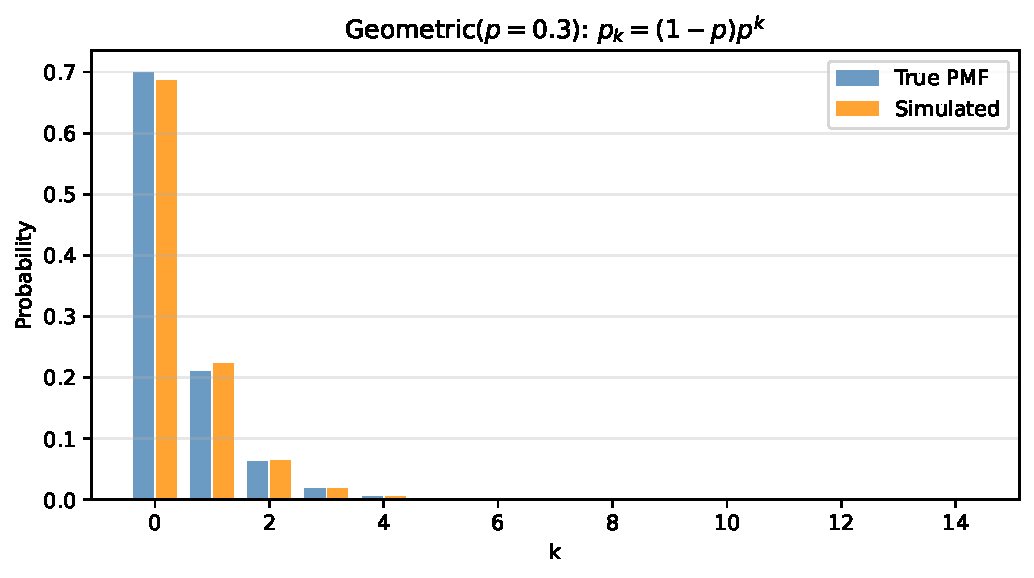
\includegraphics[width=0.55\textwidth]{fig_geometric}
    \caption{Geometric($p=0.3$) via closed-form ITM.}
  \end{figure}
\end{frame}

% ============================================================
\section{3.3 Ad Hoc Methods}
% ============================================================

\begin{frame}[allowframebreaks]{3.3.1 Binomial B$(n,p)$}
  \begin{block}{Representation as Sum of Bernoulli Trials}
    \[
      X \stackrel{\mathcal{D}}{=} \sum_{j=1}^{n} \xi_j,
    \]
    where $\xi_1,\ldots,\xi_n$ are i.i.d.\ with $\PP(\xi_j=1)=p$.
  \end{block}

  \textbf{Algorithm 11 (DB):}
  \begin{enumerate}
    \item $X \leftarrow 0$
    \item \textbf{for} $i=1$ \textbf{to} $n$:
    \begin{itemize}
      \item Generate $U\sim\UU[0,1)$
      \item \textbf{if} $U\le p$: $X \leftarrow X+1$
    \end{itemize}
    \item \textbf{return} $X$
  \end{enumerate}

  \medskip
  This is $O(n)$.  For large $n$ with moderate $np$, the ITR algorithm
  (based on the recursion) is faster.

  \framebreak

  \begin{block}{3.3.2 Erlang Distribution $\mathrm{Erl}(n,\lambda)$}
    $X = Y_1 + \cdots + Y_n$ where $Y_i \stackrel{\text{i.i.d.}}{\sim} \mathrm{Exp}(\lambda)$.

    \medskip
    Since $Y_i = -\log(U_i)/\lambda$:
    \[
      X = -\frac{1}{\lambda}\log(U_1\cdots U_n) = -\frac{\log(\prod_{i=1}^n U_i)}{\lambda}.
    \]
    PDF: $f(x) = \dfrac{1}{\Gamma(n)}\lambda^n x^{n-1}e^{-\lambda x}$, $x\ge 0$.
  \end{block}

  Also: $\mathrm{Erl}(n,\lambda)$ is a special case of $\mathrm{Gamma}(n,\lambda)$.
\end{frame}

\begin{frame}{3.3.3 Poisson Distribution Poi$(\lambda)$}
  \begin{columns}
    \column{0.52\textwidth}
    \begin{block}{Renewal Process Characterisation}
      Let $\tau_1, \tau_2, \ldots$ be i.i.d.\ $\mathrm{Exp}(1)$.
      Count the number $N$ of partial sums $\le \lambda$:
      \[
        N = \max\{i\ge 1 : \tau_1 + \cdots + \tau_i \le \lambda\}.
      \]
      \textbf{Proposition 3.3.1:} $N \stackrel{\mathcal{D}}{=} \mathrm{Poi}(\lambda)$.
    \end{block}

    Simplified using $\tau_i = -\log U_i$:
    \[
      N = \max\!\left\{n\ge 0 : \prod_{i=1}^n U_i \ge e^{-\lambda}\right\}.
    \]
    (\textit{convention:} empty product $= 1$.)

    \column{0.46\textwidth}
    \textbf{Algorithm 12 (DP):}
    \begin{enumerate}
      \item $X\leftarrow 0$, $U\sim\UU[0,1)$, $S\leftarrow -\log U$
      \item \textbf{while} $S < \lambda$:
      \begin{itemize}
        \item $U\sim\UU[0,1)$
        \item $S \leftarrow S - \log U$
        \item $X \leftarrow X+1$
      \end{itemize}
      \item \textbf{return} $X$
    \end{enumerate}

    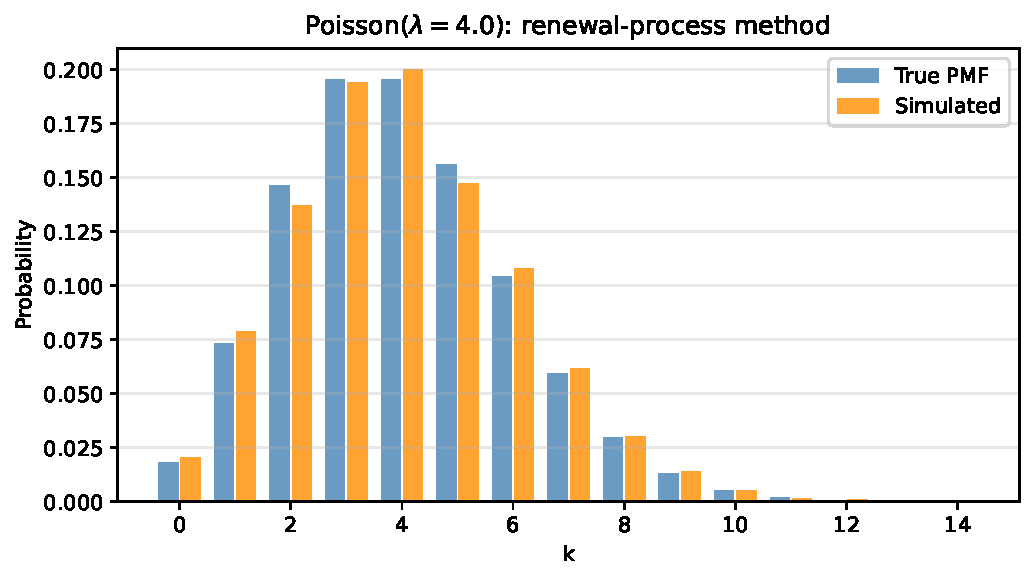
\includegraphics[width=\textwidth]{fig_poisson}
  \end{columns}
\end{frame}

\begin{frame}[fragile]{3.3 Python Code: Poisson and Erlang}
  \begin{lstlisting}[style=python, caption={Ad hoc methods for Poisson and Erlang}]
import numpy as np
rng = np.random.default_rng(0)

def sample_poisson(lam, rng):
    """Renewal-process algorithm for Poi(lam)."""
    U = rng.uniform()
    S = -np.log(U)
    X = 0
    while S < lam:
        U = rng.uniform()
        S -= np.log(U)
        X += 1
    return X

def sample_erlang(n, lam, rng):
    """Sum of n Exp(lam) variables for Erl(n, lam)."""
    U = rng.uniform(0, 1, n)
    return -np.log(np.prod(U)) / lam   # numerically stable for small n

# Example
samples_poi = [sample_poisson(3.5, rng) for _ in range(10000)]
samples_erl = [sample_erlang(4, 1.0, rng) for _ in range(10000)]
print(f"Poi(3.5) mean = {np.mean(samples_poi):.3f} (theory: 3.5)")
print(f"Erl(4,1) mean = {np.mean(samples_erl):.3f} (theory: 4.0)")
  \end{lstlisting}
\end{frame}

% ============================================================
\section{3.4 Uniform Distribution on Geometric Shapes}
% ============================================================

\begin{frame}[allowframebreaks]{3.4 Uniform Distribution on Subsets of $\RR^d$}
  A random vector $\mathbf{X}\in A\subset\RR^d$ is \emph{uniformly distributed}
  $\UU(A)$ if:
  \[
    \PP(\mathbf{X}\in D) = \frac{\Vol D}{\Vol A}, \quad D\subset A.
  \]
  Equivalently, $f(\mathbf{x}) = \frac{1}{\Vol A}\mathbf{1}(\mathbf{x}\in A)$.

  \medskip
  \textbf{Linear transform:} If $V\sim\UU(a,b)$ is needed, use $V=(b-a)U+a$
  where $U\sim\UU[0,1)$.

  \medskip
  \begin{block}{Proposition 3.4.1 --- Rejection for Subsets}
    If $A\subset B$ and $\mathbf{X}\sim\UU(B)$, then
    $(\mathbf{X}\mid\mathbf{X}\in A)\sim\UU(A)$.
  \end{block}

  \framebreak

  \textbf{Algorithm 13} $\UU(A)$:
  \begin{enumerate}
    \item Generate i.i.d.\ $U_1,\ldots,U_d\sim\UU[0,1)$
    \item $V_i \leftarrow (b_i-a_i)U_i + a_i$ (transform to bounding box)
    \item \textbf{if} $\mathbf{V}=(V_1,\ldots,V_d)\in A$: $\mathbf{X}=\mathbf{V}$; else go to 1
    \item \textbf{return} $\mathbf{X}$
  \end{enumerate}

  \medskip
  \begin{alertblock}{Curse of Dimensionality for Balls}
    The $d$-ball $B_d = \{\mathbf{x}:\sum x_i^2\le 1\}$ has volume
    $\Vol B_d = \pi^{d/2}/\Gamma(d/2+1)$.
    The $d$-cube $A_d=[-1,1]^d$ has volume $2^d$.

    \medskip
    Acceptance probability $= \Vol B_d / 2^d$.
    By Stirling: $\approx \frac{1}{\sqrt{\pi k}}\!\left(\frac{\pi e}{4k}\right)^k\to 0$
    exponentially fast (e.g., $\approx 2\times 10^{-14}$ for $d=30$).
  \end{alertblock}

  \textbf{Conclusion:} Rejection method is impractical for high-dimensional balls.
  Better algorithms use the Normal-distribution trick (Section 3.8).
\end{frame}

% ============================================================
\section{3.5 Acceptance-Rejection Method}
% ============================================================

\begin{frame}[allowframebreaks]{3.5.1 AR-d (Discrete Acceptance-Rejection)}
  \textbf{Setting:} Want $X\sim(p_j)_{j\in E}$.  We can easily sample $Y\sim(q_j)_{j\in E}$.
  There exists $c>0$ such that
  \[
    p_j \le c\,q_j \quad \forall j\in E.
  \]

  \begin{block}{Proposition 3.5.1 --- AR Correctness}
    Define the acceptance region $A = \{cUq_Y \le p_Y\}$ for independent
    $U\sim\UU[0,1)$ and $Y\sim(q_j)$.  Then:
    \[
      \PP(A) = 1/c \quad\text{and}\quad \PP(Y=j\mid A) = p_j.
    \]
  \end{block}

  \begin{alertblock}{Algorithm 14 --- AR-d}
    \textbf{Require:} $c>0$ with $p_j\le cq_j$; algorithm to sample $Y\sim(q_j)$.\\
    \textbf{Ensure:} $X\sim(p_j)$.
    \begin{enumerate}
      \item \textbf{repeat}
      \begin{itemize}
        \item Generate $Y\sim(q_j)$ and $U\sim\UU[0,1)$ (independent)
      \end{itemize}
      \item \textbf{until} $cUq_Y \le p_Y$
      \item \textbf{return} $X=Y$
    \end{enumerate}
    Expected number of iterations $= c$.  Choose the \emph{smallest} possible $c$.
  \end{alertblock}

  \framebreak

  \textbf{Example 3.5.2:} Sample $X$ with $p_j = \frac{6}{\pi^2 j^2}$, $j=1,2,\ldots$

  Proposal: $q_j = \frac{1}{j(j+1)}$ (can be sampled as $Y=\lfloor U^{-1}\rfloor$).

  \[
    \frac{p_j}{q_j} = \frac{6}{\pi^2 j^2} \cdot j(j+1) = \frac{6}{\pi^2}\frac{j+1}{j}.
  \]

  $c = \sup_j(p_j/q_j) = 12/\pi^2$.

  \medskip
  Acceptance condition:
  \[
    cUq_Y \le p_Y \iff 2UY \le Y+1.
  \]
\end{frame}

\begin{frame}[allowframebreaks]{3.5.2 AR-c (Continuous Acceptance-Rejection)}
  \textbf{Setting:} Want $X$ with p.d.f.\ $f(x)$ on $E$.
  Can sample $Y$ with p.d.f.\ $g(x)$.
  There exists $c<\infty$ such that $f(x)\le cg(x)$ for all $x\in E$.

  \begin{block}{Proposition 3.5.3 --- AR-c Correctness}
    \[
      \PP(A) = 1/c \quad\text{and}\quad \PP(Y\in B\mid A) = \int_B f(y)\,dy.
    \]
  \end{block}

  \begin{alertblock}{Algorithm 16 --- AR-c}
    \textbf{Require:} $c>0$ with $f(x)\le cg(x)$; algorithm to sample $Y\sim g$.\\
    \textbf{Ensure:} $X\sim f$.
    \begin{enumerate}
      \item \textbf{repeat}
      \begin{itemize}
        \item Generate $Y\sim g$ and $U\sim\UU[0,1]$ (independent)
      \end{itemize}
      \item \textbf{until} $cUg(Y)\le f(Y)$
      \item \textbf{return} $X=Y$
    \end{enumerate}
  \end{alertblock}

  \framebreak

  \begin{block}{Example 3.5.4 --- Normal from Exponential (AR-N)}
    Half-normal target: $f(x) = \frac{2}{\sqrt{2\pi}}e^{-x^2/2}$, $x>0$.

    Proposal: $g(x) = e^{-x}$ (i.e., $Y\sim\mathrm{Exp}(1)$).

    Optimal constant:
    \[
      c = \max_{x>0}\frac{f(x)}{g(x)} = \sqrt{\frac{2e}{\pi}} \approx 1.32.
    \]
    Acceptance condition (after simplification):
    \[
      U \le \exp\!\left(-\frac{(Y-1)^2}{2}\right).
    \]
    Then draw sign $I = \pm 1$ with probability $1/2$ each; return $Z = IY$.
  \end{block}

  \begin{figure}
    \centering
    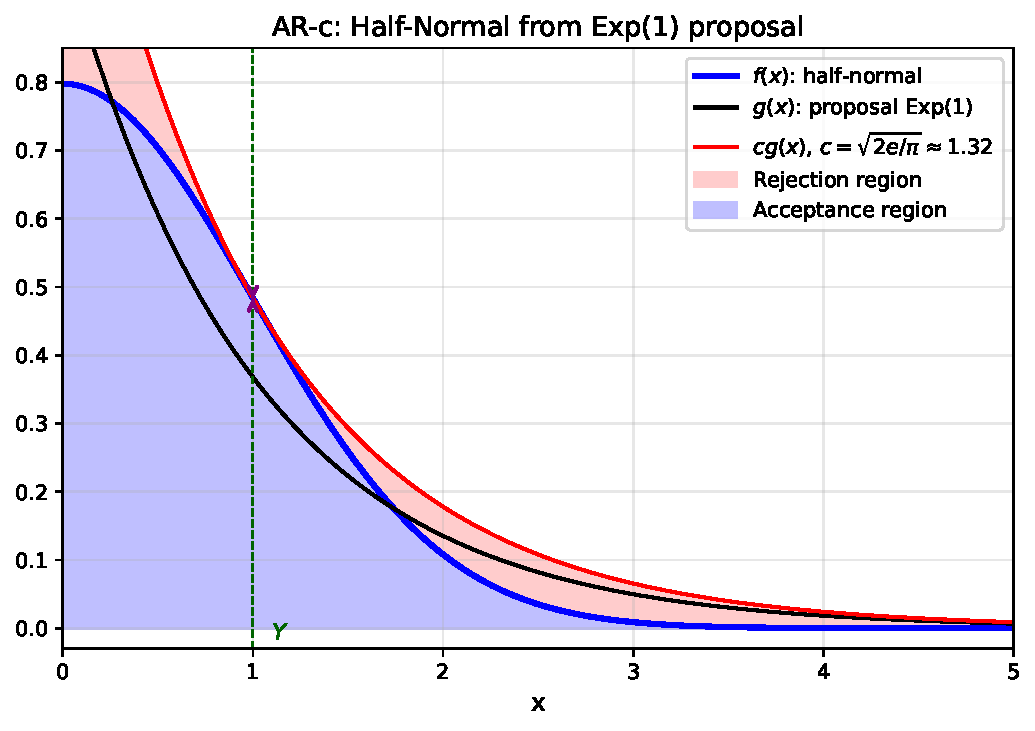
\includegraphics[width=0.6\textwidth]{fig_ar_halfnormal}
    \caption{Half-normal density $f$, proposal $g\sim\mathrm{Exp}(1)$,
      and envelope $cg$. Red area is rejected; blue area is accepted.}
  \end{figure}
\end{frame}

\begin{frame}[fragile]{3.5 Python Code: AR-c for Normal}
  \begin{lstlisting}[style=python, caption={AR-c to generate N(0,1) via half-normal and Exp(1)}]
import numpy as np
rng = np.random.default_rng(42)

def sample_normal_arc(n, rng):
    """Algorithm 17 AR-N: generate N(0,1) via AR-c."""
    out = np.empty(n)
    i = 0
    while i < n:
        U1 = rng.uniform()
        Y  = -np.log(U1)          # Y ~ Exp(1)
        U2 = rng.uniform()
        if U2 <= np.exp(-(Y - 1)**2 / 2):   # acceptance condition
            sign = 1 if rng.uniform() < 0.5 else -1
            out[i] = sign * Y
            i += 1
    return out

Z = sample_normal_arc(5000, rng)
print(f"Mean: {Z.mean():.4f}  (theory: 0)")
print(f"Std:  {Z.std():.4f}   (theory: 1)")
  \end{lstlisting}

  \medskip
  \textbf{Unknown normalising constants:}  When $f(x)=f^*(x)/c_f$ and
  $g(x)=g^*(x)/c_g$, the acceptance condition $U\le f^*(Y)/(c^*g^*(Y))$ still works,
  where $c^*=\sup f^*(x)/g^*(x)$.  No need to know $c_f$ or $c_g$ separately.
\end{frame}

% ============================================================
\section{3.6 Composition Method}
% ============================================================

\begin{frame}[allowframebreaks]{3.6 Composition (Mixture) Method}
  \begin{block}{Setup}
    Suppose
    \[
      f(x) = \sum_{j=1}^{n} p_j\, g_j(x),
    \]
    where $g_j$ are p.d.f.s and $(p_j)$ is a probability function
    ($p_j\ge 0$, $\sum p_j=1$).  $f$ is then a \emph{mixture distribution}.
  \end{block}

  \begin{alertblock}{Composition Algorithm}
    \begin{enumerate}
      \item Sample component index $J$ with $\PP(J=j)=p_j$.
      \item Given $J=j$, generate $X\sim g_j$.
      \item \textbf{return} $X$.
    \end{enumerate}
    Works for infinite mixtures too:
    $f(x) = \sum_{j=0}^\infty p_j g_j(x)$.
  \end{alertblock}

  \begin{figure}
    \centering
    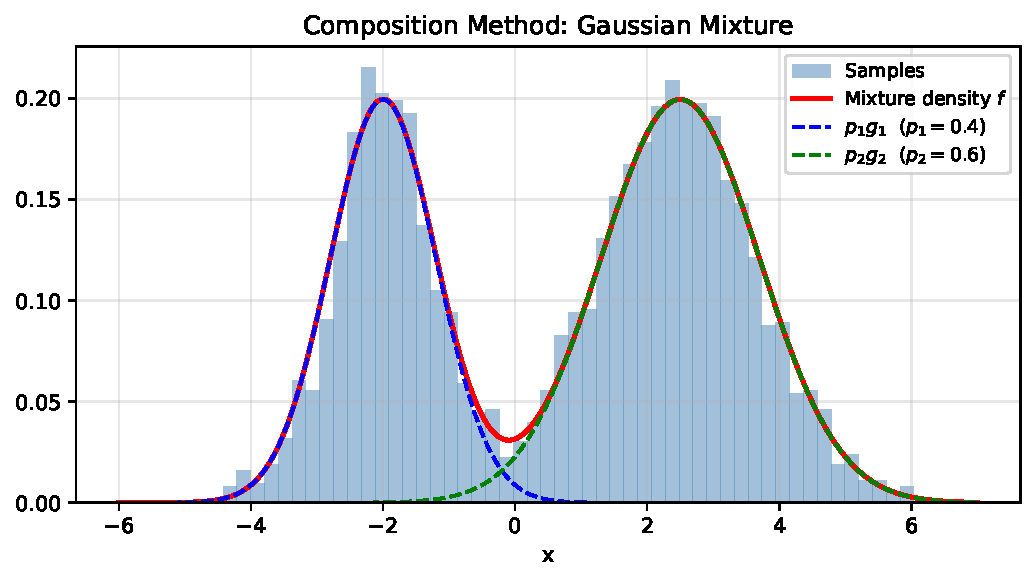
\includegraphics[width=0.55\textwidth]{fig_composition}
    \caption{Gaussian mixture $f = p_1 g_1 + p_2 g_2$ via composition method.}
  \end{figure}

  \framebreak

  \textbf{Example 3.6.1 --- Non-central Chi-square:}
  \[
    f(x) = \tfrac{1}{2}e^{-(x+\lambda)/2}\!\left(\tfrac{x}{\lambda}\right)^{d/4-1/2}\!
            I_{d/2-1}(\sqrt{\lambda x}), \quad x\ge 0.
  \]
  Can be represented as a mixture of $\mathrm{Gamma}(j+d/2, 1/2)$ distributions
  with Poisson$(\lambda/2)$ mixing weights.

  \medskip
  \textbf{Example 3.6.3 --- Gamma-Poisson (Negative Binomial) mixture:}

  If $X\mid\Lambda\sim\mathrm{Poi}(\Lambda)$ and
  $\Lambda\sim\mathrm{Gamma}(\alpha,\lambda)$, then
  \[
    X\sim\mathrm{NB}\!\left(\alpha,\,\tfrac{1}{1+\lambda}\right).
  \]
  This is the \emph{Gamma-Poisson mixture} representation.
\end{frame}

\begin{frame}[fragile]{3.6 Python Code: Mixture Sampling}
  \begin{lstlisting}[style=python, caption={Composition method for Gaussian mixture}]
import numpy as np
rng = np.random.default_rng(0)

def sample_mixture(p, mus, sigmas, n, rng):
    """
    Composition method for Gaussian mixture.
    p      : list of mixture weights (sum to 1)
    mus    : list of means
    sigmas : list of std devs
    """
    p = np.array(p)
    # Step 1: sample component index
    J = rng.choice(len(p), size=n, p=p)
    # Step 2: sample from chosen component
    X = np.array([rng.normal(mus[j], sigmas[j]) for j in J])
    return X

p     = [0.3, 0.5, 0.2]
mus   = [-3.0, 1.0, 5.0]
sigmas= [0.8,  1.2, 0.5]
X = sample_mixture(p, mus, sigmas, n=10000, rng=rng)
print(f"Empirical mean: {X.mean():.3f}")
# Theory: 0.3*(-3) + 0.5*1 + 0.2*5 = 0.6
  \end{lstlisting}
\end{frame}

% ============================================================
\section{3.7 Generating Gaussian Random Numbers}
% ============================================================

\begin{frame}[allowframebreaks]{3.7.1 Box-Muller Method}
  \begin{block}{Lemma 3.7.1 --- Polar Representation of Bivariate Normal}
    Let $Z_1, Z_2$ be i.i.d.\ $\NN(0,1)$.  Let $(D,\Theta)$ be their
    polar coordinates.  Then:
    \begin{itemize}
      \item $D$ and $\Theta$ are \emph{independent},
      \item $D$ has p.d.f.\ $f(r) = r e^{-r^2/2}$ (Rayleigh distribution),
      \item $\Theta\sim\UU[0,2\pi)$.
    \end{itemize}
  \end{block}

  \begin{block}{Lemma 3.7.2 --- Rayleigh Distribution}
    If $D$ has the Rayleigh distribution, then $Y=D^2\sim\mathrm{Exp}(1/2)$.
    Thus $D \stackrel{\mathcal{D}}{=} (-2\log U)^{1/2}$.
  \end{block}

  \begin{alertblock}{Proposition 3.7.3 --- Box-Muller}
    Let $U_1,U_2\stackrel{\text{i.i.d.}}{\sim}\UU[0,1)$.  Set
    \[
      Z_1 = (-2\log U_1)^{1/2}\cos(2\pi U_2), \quad
      Z_2 = (-2\log U_1)^{1/2}\sin(2\pi U_2).
    \]
    Then $Z_1, Z_2$ are i.i.d.\ $\NN(0,1)$.
  \end{alertblock}

  \framebreak

  \textbf{Algorithm 20 (BM):}
  \begin{enumerate}
    \item Generate $U_1,U_2$ i.i.d.\ $\UU[0,1)$
    \item $D\leftarrow -2\log U_1$, $V\leftarrow 2\pi U_2$
    \item $Z_1=\sqrt{D}\cos V$, $Z_2=\sqrt{D}\sin V$
    \item \textbf{return} $Z_1, Z_2$
  \end{enumerate}

  \begin{figure}
    \centering
    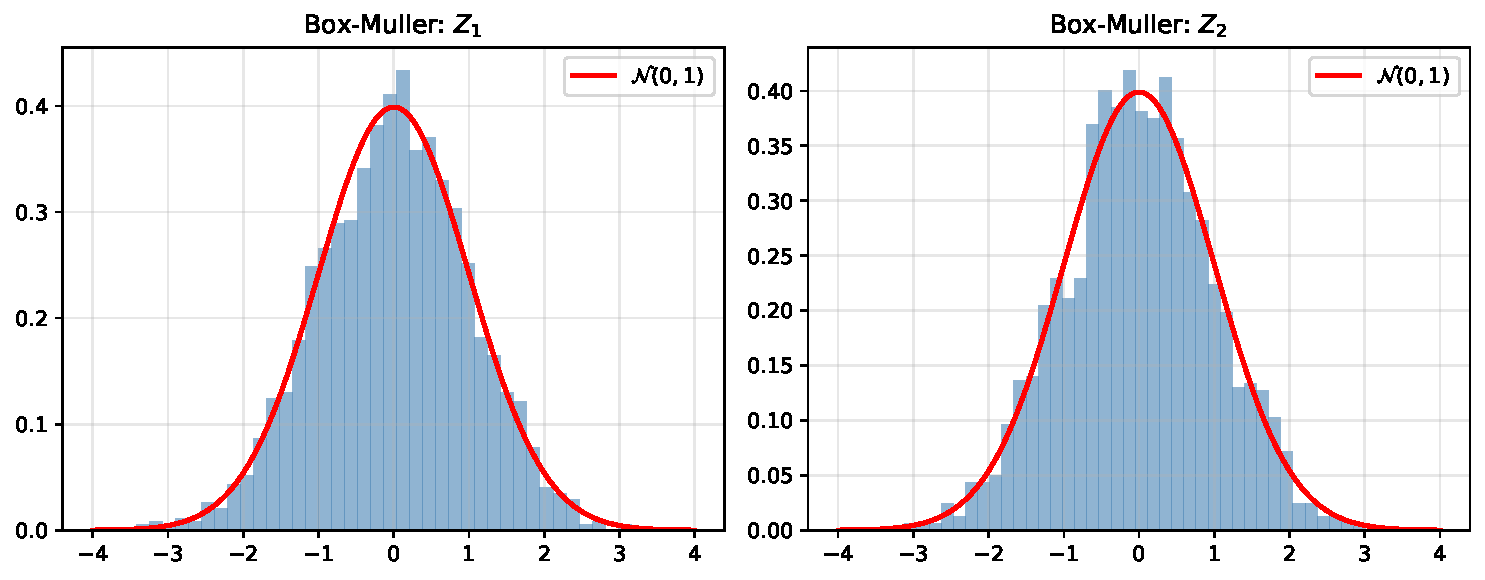
\includegraphics[width=0.65\textwidth]{fig_box_muller}
    \caption{Box-Muller: histograms of $Z_1$ and $Z_2$ vs $\NN(0,1)$ density.}
  \end{figure}
\end{frame}

\begin{frame}[allowframebreaks]{3.7.1 Marsaglia-Bray Method}
  \begin{block}{Proposition 3.7.4 --- Marsaglia-Bray}
    Let $V_1,V_2\stackrel{\text{i.i.d.}}{\sim}\UU[-1,1)$.  Set
    $Y_i = (-2\log(V_1^2+V_2^2))^{1/2} V_i/(V_1^2+V_2^2)^{1/2}$.

    Conditional on $V_1^2+V_2^2\le 1$:
    $(Z_1,Z_2) = (Y_1,Y_2) \stackrel{\mathcal{D}}{=}$ i.i.d.\ $\NN(0,1)$.
  \end{block}

  \textbf{Algorithm 21 (MB):}
  \begin{enumerate}
    \item \textbf{repeat}: $U_1,U_2$ i.i.d.\ $\UU[0,1)$;
      $V_1=2U_1-1$, $V_2=2U_2-1$; $X'=V_1^2+V_2^2$
    \item \textbf{until} $X'\le 1$
    \item $Y\leftarrow\sqrt{-2\log(X')/X'}$
    \item $Z_1=V_1\cdot Y$, $Z_2=V_2\cdot Y$
  \end{enumerate}

  \textbf{Acceptance probability} $\approx \pi/4 \approx 78.5\%$.

  \medskip
  \textbf{Advantage over Box-Muller:}
  Avoids trigonometric functions; generally faster in practice.

  \begin{figure}
    \centering
    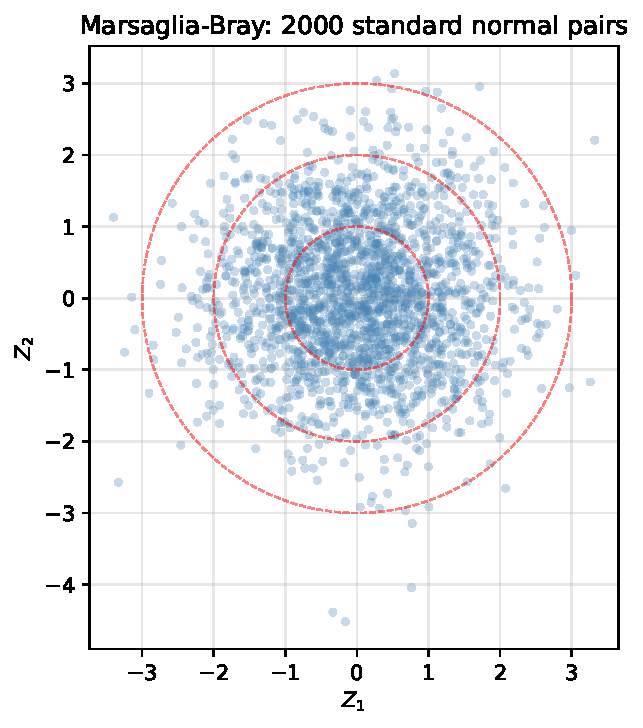
\includegraphics[width=0.45\textwidth]{fig_marsaglia_bray}
    \caption{2000 standard normal pairs from Marsaglia-Bray.}
  \end{figure}
\end{frame}

\begin{frame}[fragile]{3.7.2 ITM for Normal Variables}
  To generate $\NN(0,1)$ via ITM, invert the c.d.f.\ $\Phi$.
  No closed form for $\Phi^{-1}(u)$; use numerical methods.

  \begin{block}{Newton's Method}
    Solve $\Phi(x)=u$ starting from $x_0=\pm\sqrt{|-1.6\log(1.0004-(1-2u)^2)|}$:
    \[
      x_{n+1} = x_n + (u - \Phi(x_n))e^{0.5x_n^2+c}, \quad c=\log\sqrt{2\pi}.
    \]
    One additional step reduces error to below $10^{-15}$.
  \end{block}

  \begin{lstlisting}[style=python, caption={Inverse normal c.d.f.\ via scipy}]
from scipy.stats import norm
import numpy as np

# scipy.stats.norm.ppf implements the Beasley-Springer-Moro algorithm
p = 0.95
quantile = norm.ppf(p)
print(f"Phi^(-1)(0.95) = {quantile:.6f}")  # 1.644854

# Generate N(0,1) samples via ITM
rng = np.random.default_rng(42)
U = rng.uniform(0, 1, 5000)
Z = norm.ppf(U)      # inverse CDF method
print(f"Mean: {Z.mean():.4f}, Std: {Z.std():.4f}")
  \end{lstlisting}
\end{frame}

\begin{frame}[allowframebreaks]{3.7.3 Generating Multivariate Normal $\NN(\boldsymbol{\mu},\boldsymbol{\Sigma})$}
  \begin{block}{Cholesky Factorisation Method}
    Every symmetric positive-semidefinite matrix $\boldsymbol{\Sigma}$ admits
    \[
      \boldsymbol{\Sigma} = \mathbf{A}\mathbf{A}^T.
    \]
    (Cholesky gives lower-triangular $\mathbf{A}$.)

    \medskip
    \textbf{Proposition 3.7.8:} Let $\mathbf{Z}=(Z_1,\ldots,Z_d)^T$, i.i.d.\ $\NN(0,1)$.
    Then
    \[
      \mathbf{X} = \mathbf{A}\mathbf{Z} + \boldsymbol{\mu} \sim \NN(\boldsymbol{\mu},\boldsymbol{\Sigma}).
    \]
    \textit{Proof:} $\EE[\mathbf{X}]=\boldsymbol{\mu}$ and
    $\mathrm{Cov}(\mathbf{X})=\mathbf{A}\mathbf{Id}\,\mathbf{A}^T=\boldsymbol{\Sigma}$.
  \end{block}

  \begin{block}{Bivariate Case ($d=2$)}
    With $\boldsymbol{\Sigma}=\begin{pmatrix}\sigma_1^2 & \rho\sigma_1\sigma_2\\
    \rho\sigma_1\sigma_2 & \sigma_2^2\end{pmatrix}$:
    \[
      X_1 = \sigma_1(\sqrt{1-|\rho|}Z_1 + \sqrt{|\rho|}Z_3),\quad
      X_2 = \sigma_2(\sqrt{1-|\rho|}Z_2 + \mathrm{sign}(\rho)\sqrt{|\rho|}Z_3).
    \]
  \end{block}

  \framebreak

  \begin{figure}
    \centering
    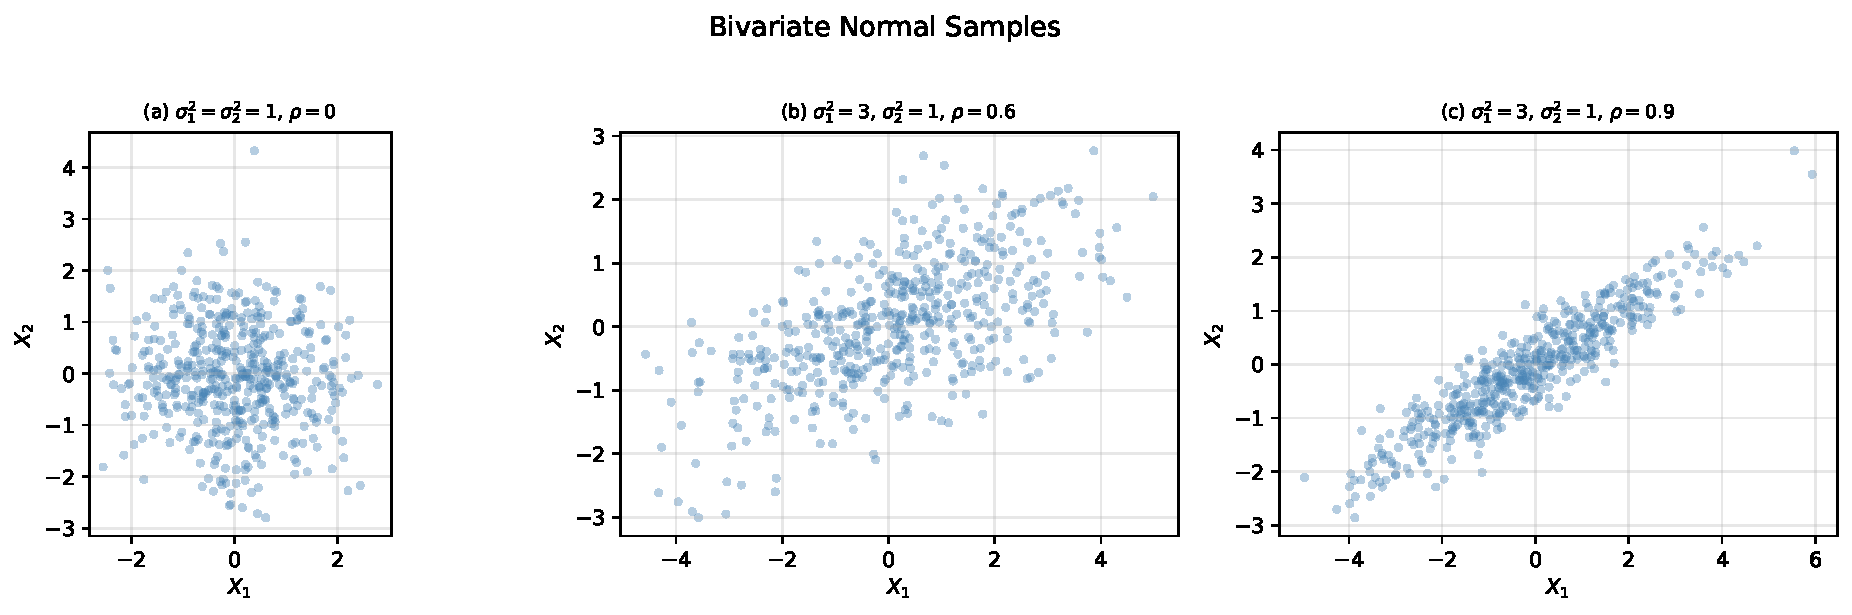
\includegraphics[width=0.85\textwidth]{fig_bivariate_normal}
    \caption{500 samples from bivariate normal under three different covariance settings.}
  \end{figure}
\end{frame}

\begin{frame}[fragile]{3.7.3 Python: Multivariate Normal via Cholesky}
  \begin{lstlisting}[style=python, caption={Generate multivariate normal via Cholesky decomposition}]
import numpy as np
rng = np.random.default_rng(42)

def sample_multivariate_normal(mu, Sigma, n, rng):
    """Generate n samples from N(mu, Sigma) via Cholesky."""
    d = len(mu)
    A = np.linalg.cholesky(Sigma)   # Sigma = A @ A.T
    Z = rng.standard_normal((d, n))  # d x n matrix of i.i.d. N(0,1)
    return (A @ Z).T + mu            # n x d output

# Example: 2D normal with correlation 0.8
mu    = np.array([1.0, -2.0])
Sigma = np.array([[2.0, 1.2],
                  [1.2, 1.0]])       # rho = 1.2/sqrt(2) ? 0.849
samples = sample_multivariate_normal(mu, Sigma, 2000, rng)
print("Empirical mean:", samples.mean(axis=0).round(3))
print("Empirical cov:\n", np.cov(samples.T).round(3))
  \end{lstlisting}
\end{frame}

% ============================================================
\section{3.8 Uniform Distribution on Balls, Spheres, Ellipsoids}
% ============================================================

\begin{frame}[allowframebreaks]{3.8 Geometric Setup}
  \textbf{Objects:}
  \begin{align*}
    B_d &= \{\mathbf{x}\in\RR^d : x_1^2+\cdots+x_d^2\le 1\},
      \quad \Vol(B_d) = \frac{\pi^{d/2}}{\Gamma(d/2+1)}, \\[4pt]
    S_{d-1} &= \{\mathbf{x}\in\RR^d : x_1^2+\cdots+x_d^2 = 1\},
      \quad \mathrm{Area}(S_{d-1}) = \frac{d\pi^{d/2}}{\Gamma(d/2+1)}.
  \end{align*}

  \begin{block}{Change of Variables --- Key Formula}
    For a parametrised surface $\mathbf{x}(\mathbf{t})$ with Jacobian matrix
    $\mathbf{J}(\mathbf{t}) = (\partial x_j/\partial t_i)_{i,j}$:
    \[
      \sqrt{g(\mathbf{t})} = \sqrt{|\det(\mathbf{J}\mathbf{J}^T)|}.
    \]
    Surface area element: $dA = \sqrt{g(\mathbf{t})}\,d\mathbf{t}$.
  \end{block}

  \framebreak

  \begin{block}{3.8.1 Random Point in $B_3$ and on $S_2$}
    Spherical coordinates for $B_3$:
    $x = r\cos\theta\sin\phi$, $y=r\sin\theta\sin\phi$, $z=r\cos\phi$.

    \medskip
    \textbf{Proposition 3.8.4:} For $\mathbf{X}\sim\UU(B_3)$ in spherical coords $(D,\Phi,\Theta)$:
    \begin{itemize}
      \item $D^{1/3}\sim\UU[0,1)$ (so $D\stackrel{\mathcal{D}}{=}U^{1/3}$),
      \item $\Phi = \arccos(1-2U')$, $U'\sim\UU[0,1)$,
      \item $\Theta\sim\UU[0,2\pi)$.
    \end{itemize}

    \medskip
    \textbf{Proposition 3.8.6:} If $Z_1,Z_2,Z_3\stackrel{\text{i.i.d.}}{\sim}\NN(0,1)$:
    \[
      \left(\frac{Z_1}{\|\mathbf{Z}\|},\frac{Z_2}{\|\mathbf{Z}\|},\frac{Z_3}{\|\mathbf{Z}\|}\right)
      \sim\UU(S_2).
    \]
    \textbf{Proposition 3.8.13:} If $\mathbf{X}\sim\UU(S_{d-1})$ and
    $U\sim\UU[0,1)$ independent, then $U^{1/d}\mathbf{X}\sim\UU(B_d)$.
  \end{block}

  \begin{figure}
    \centering
    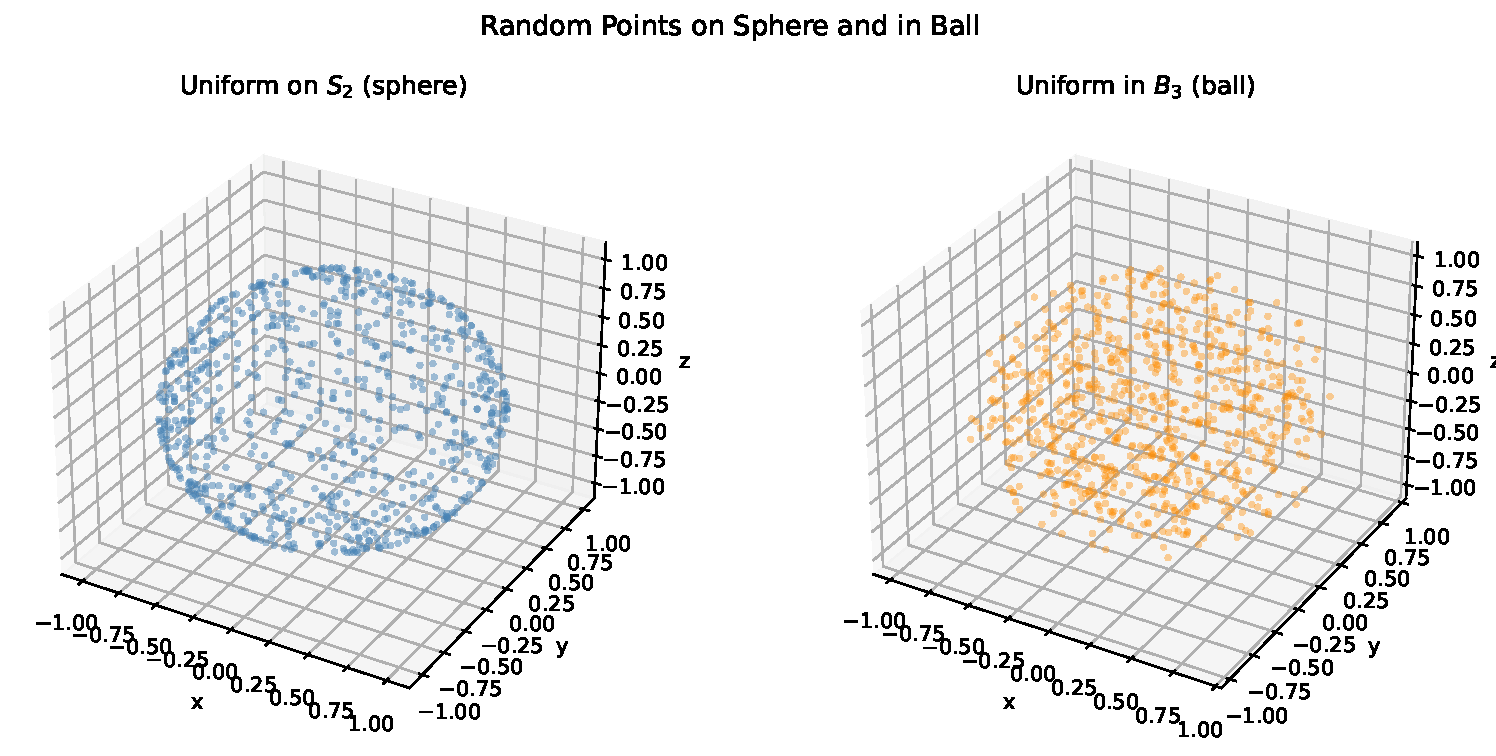
\includegraphics[width=0.60\textwidth]{fig_ball_sphere}
    \caption{Uniform random points on $S_2$ (left) and in $B_3$ (right).}
  \end{figure}
\end{frame}

\begin{frame}[fragile]{3.8 Python: Sphere and Ball Sampling}
  \begin{lstlisting}[style=python, caption={Sample uniformly from sphere and ball in d dimensions}]
import numpy as np
rng = np.random.default_rng(42)

def sample_sphere(d, n, rng):
    """Uniform on (d-1)-sphere S_{d-1} by normalising N(0,I)."""
    Z = rng.standard_normal((n, d))
    return Z / np.linalg.norm(Z, axis=1, keepdims=True)

def sample_ball(d, n, rng):
    """Uniform in d-ball B_d: X = U^{1/d} * point_on_sphere."""
    X = sample_sphere(d, n, rng)
    U = rng.uniform(0, 1, n)
    return X * U[:, None]**(1.0/d)

# 3D examples
pts_sphere = sample_sphere(3, 1000, rng)
pts_ball   = sample_ball(3, 1000, rng)
print("Sphere norms:", np.linalg.norm(pts_sphere, axis=1).mean().round(4))  # ~1
print("Ball norms:  ", np.linalg.norm(pts_ball,   axis=1).mean().round(4))  # ~0.75
  \end{lstlisting}
\end{frame}

\begin{frame}[allowframebreaks]{3.8.2--3.8.3 Spherical Coordinates \& Ellipsoids}
  \begin{block}{3.8.2 General Spherical Coordinates in $\RR^d$}
    \[
      x_1 = r\cos\phi_1, \quad x_2 = r\sin\phi_1\cos\phi_2, \quad \ldots
    \]
    Jacobian: $J = r^{d-1}\sin^{d-2}\phi_1\sin^{d-3}\phi_2\cdots\sin\phi_{d-2}$.

    \medskip
    \textbf{Lemma 3.8.10:} For $\mathbf{Z}\sim\NN(\mathbf{0},\mathbf{Id})$, the
    spherical coordinates $(D,\Phi_1,\ldots,\Phi_{d-2},\Theta)$ are independent,
    $D^2\sim\chi^2_d$, and $\Phi_i$ has p.d.f.\ $c_{d-i-1}\sin^{d-i-1}x$.
  \end{block}

  \begin{block}{3.8.3 Ellipsoids}
    A $d$-ellipsoid: $\mathcal{E}_d = \{\mathbf{x}\in\RR^d : \mathbf{x}^T\mathbf{A}^{-1}\mathbf{x}\le 1\}$
    where $\mathbf{A}$ is symmetric positive-definite.

    \medskip
    Factorize $\mathbf{A} = \mathbf{L}\mathbf{L}^T$.

    \medskip
    \textbf{Algorithm 23:}
    \begin{enumerate}
      \item Diagonalize $\mathbf{A}=\mathbf{P}\,\mathrm{diag}(\mathbf{a}^2)\,\mathbf{P}^T$
      \item $\mathbf{L}\leftarrow\mathbf{P}\,\mathrm{diag}(\mathbf{a})$
      \item Generate $\mathbf{X}\sim\UU(B_d)$
      \item $\mathbf{Y}\leftarrow\mathbf{L}\mathbf{X}$
      \item \textbf{return} $\mathbf{Y}$
    \end{enumerate}
  \end{block}
\end{frame}

\begin{frame}[allowframebreaks]{3.8.4--3.8.5 Sampling on an Ellipsoid Surface}
  \textbf{Problem:} Sample uniformly from the surface of the ellipsoid
  $\frac{x^2}{a^2}+\frac{y^2}{b^2}+\frac{z^2}{c^2}=1$.

  \medskip
  Parametrisation: $\mathbf{x}(\theta,\phi) = (a\cos\theta\sin\phi,\,
  b\sin\theta\sin\phi,\,c\cos\phi)$ with
  $\theta\in[0,2\pi)$, $\phi\in[0,\pi)$.

  \[
    \sqrt{g(\phi,\theta)} = \sin\phi\!\sqrt{c^2(a^2-b^2)\cos^2\theta(\cos^2\phi-1) + a^2(b^2-c^2)\cos^2\phi + c^2}.
  \]

  Density $\propto\sqrt{g(\phi,\theta)}$ --- coordinates are \emph{not} independent
  for general $a,b,c$.

  \medskip
  \begin{block}{Numerical Approach (Algorithm 24)}
    \begin{enumerate}
      \item Build a grid of $n_k\times n_l$ parallelogram patches on the surface.
      \item Approximate each patch area using cross-products of tangent vectors.
      \item Sample a patch proportional to its area (composition method).
      \item Sample a uniform point within the chosen patch.
    \end{enumerate}
  \end{block}

  \framebreak

  \begin{block}{3.8.5 Average Shadow of a Convex 3D Body}
    For a flat face $F$ with outward normal randomly drawn from $\UU(S_2)$:
    \[
      \EE[\mathrm{Area}(\mathrm{shadow}(F))] = \frac{\mathrm{Area}(F)}{2}.
    \]
    For a convex polyhedron $B$ with faces $F_1,\ldots,F_m$:
    \[
      \EE[\mathrm{Area}(\mathrm{shadow}(B))]
      = \frac{\mathrm{Area}(\mathrm{surface}(B))}{4}.
    \]
    For a cube with edge $s$: $\EE[\mathrm{shadow}] = \frac{6s^2}{4} = \frac{3}{2}s^2$.
  \end{block}
\end{frame}

% ============================================================
\section{3.9 Bivariate Vectors: Conditional ITM and Copulas}
% ============================================================

\begin{frame}[allowframebreaks]{3.9.1 Conditional Inverse Transform Method}
  \textbf{Setup:} Joint density $f(x,y)$, marginals $f_X(x)$ and $f_Y(y)$,
  conditional c.d.f.:
  \[
    F_{Y|X=x}(y) = \frac{F_{X=x,Y}(\mathbf{x},y)}{f_X(\mathbf{x})}, \quad
    F_{X=x,Y}(\mathbf{x},y) = \int_{y_0}^y f(\mathbf{x},u)\,du.
  \]

  \begin{alertblock}{Algorithm: Conditional ITM}
    \begin{enumerate}
      \item Compute marginal c.d.f.\ $F_X$; sample $X=F_X^{-1}(U_1)$.
      \item Given $X=\mathbf{x}$, compute conditional c.d.f.\ $F_{Y|X=\mathbf{x}}$.
      \item Set $Y = F_{Y|X=\mathbf{x}}^{-1}(U_2)$, independent $U_2$.
      \item \textbf{return} $(X,Y)$.
    \end{enumerate}
  \end{alertblock}

  \begin{figure}
    \centering
    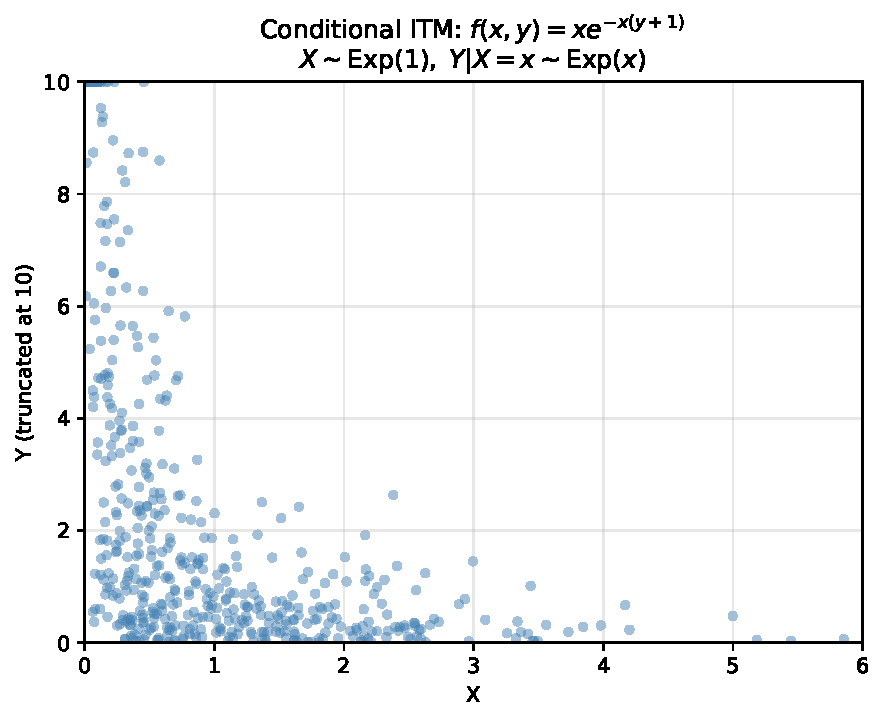
\includegraphics[width=0.45\textwidth]{fig_conditional_itm}
    \caption{100 samples from $f(x,y)=xe^{-x(y+1)}$ via conditional ITM.}
  \end{figure}

  \framebreak

  \textbf{Example 3.9.1:} $f(x,y) = x\exp(-x(y+1))$, $x,y\ge 0$.
  \begin{itemize}
    \item $f_X(x) = e^{-x}$, so $X\sim\mathrm{Exp}(1)$: $X=-\log U_1$.
    \item $f_{Y|X=x}(y) = xe^{-xy}$ (Exp$(x)$): $Y = -\log U_2 / X$.
  \end{itemize}
\end{frame}

\begin{frame}[allowframebreaks]{3.9.2 Bivariate Copulas --- Sklar's Theorem}
  \begin{block}{Definition: Copula}
    A \textbf{copula} $C(u_1,u_2)$ is any bivariate c.d.f.\ with
    $\UU[0,1)$ marginals.  Formally, $C:[0,1]^2\to[0,1]$ satisfies:
    \begin{enumerate}
      \item $C(u_i,0)=0$ and $C(u_i,1)=u_i$,
      \item $C(v_1,v_2)-C(u_1,v_2)-C(v_1,u_2)+C(u_1,u_2)\ge 0$
            for $u_i\le v_i$.
    \end{enumerate}
  \end{block}

  \begin{block}{Theorem 3.9.2 --- Sklar's Theorem}
    For any joint c.d.f.\ $F_{X,Y}(t_1,t_2)$ there exists a copula $C$ such that
    \[
      F_{X,Y}(t_1,t_2) = C(F_X(t_1),F_Y(t_2)).
    \]
    If the marginals $F_X$ and $F_Y$ are continuous, $C$ is \emph{unique}.

    \medskip
    Moreover, the joint density factors as:
    \[
      f_{X,Y}(t_1,t_2) = f_X(t_1)\,f_Y(t_2)\,c(F_X(t_1),F_Y(t_2)),
    \]
    where $c$ is the copula density.
  \end{block}

  \framebreak

  \begin{block}{Fr?chet-Hoeffding Bounds (Theorem 3.9.6)}
    For any copula $C$:
    \[
      (F(x)+F(y)-1)_+ \;\le\; F(x,y) \;\le\; \min(F(x),F(y)).
    \]
    \begin{itemize}
      \item \textbf{Upper bound} $C_U(u_1,u_2) = \min(u_1,u_2)$:
            perfect positive dependence, $V_1=V_2=U$.
      \item \textbf{Lower bound} $C_L(u_1,u_2) = \max(0,u_1+u_2-1)$:
            perfect negative dependence, $V_1=U$, $V_2=1-U$.
      \item \textbf{Independence copula} $C_I(u_1,u_2) = u_1 u_2$:
            $V_1=U_1$, $V_2=U_2$ independent.
    \end{itemize}
  \end{block}

  \begin{figure}
    \centering
    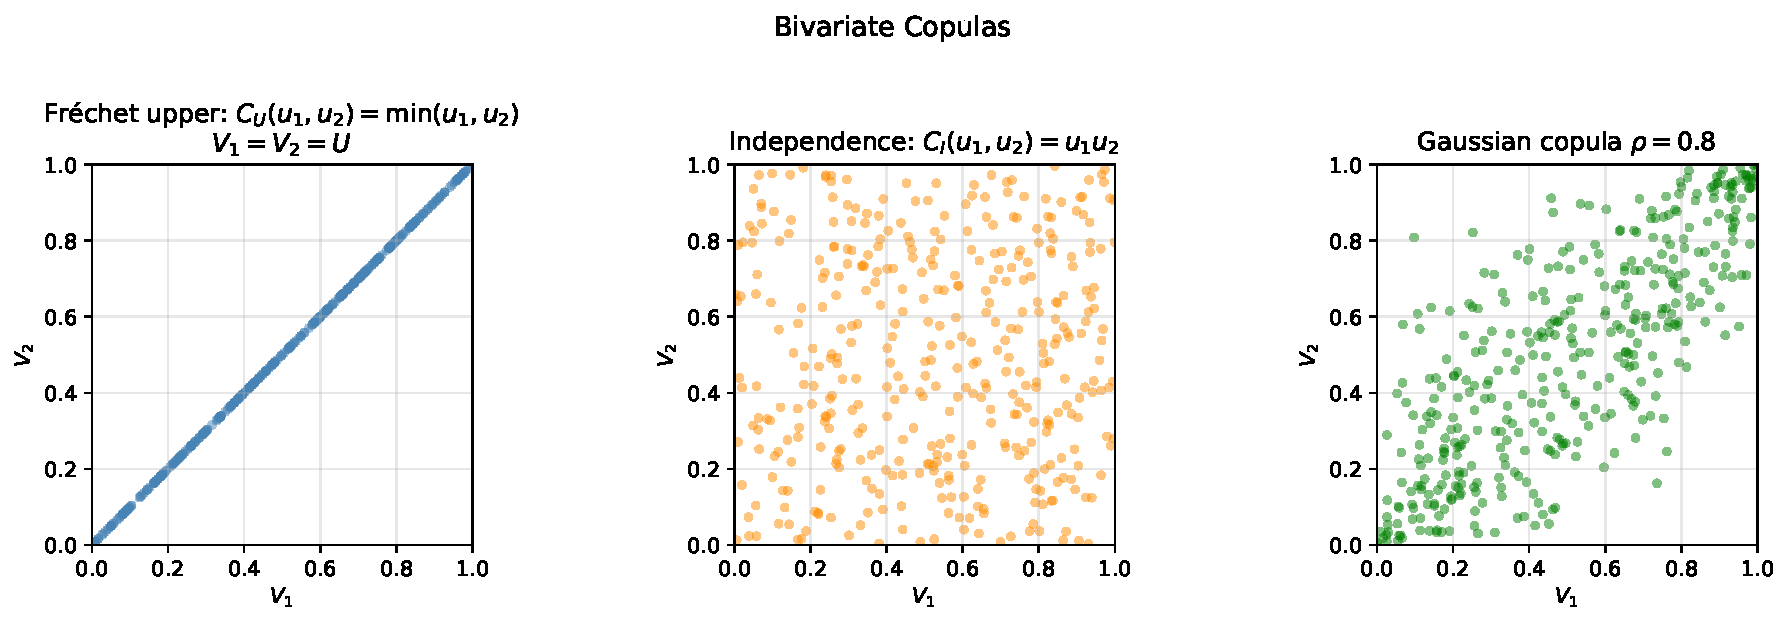
\includegraphics[width=0.75\textwidth]{fig_copulas}
    \caption{Fr?chet upper, independence, and Gaussian ($\rho=0.8$) copula samples.}
  \end{figure}
\end{frame}

\begin{frame}[allowframebreaks]{3.9.3 Classical Copulas}
  \begin{block}{Gaussian (Normal) Copula}
    Let $\Phi_\rho$ be the bivariate normal c.d.f.\ with correlation $\rho$:
    \[
      C(u_1,u_2) = \Phi_\rho(\Phi^{-1}(u_1),\Phi^{-1}(u_2)).
    \]
    \textbf{Simulation:} Generate $(X,Y)\sim\NN(\mathbf{0},\boldsymbol{\Sigma})$
    with $\boldsymbol{\Sigma}=\bigl(\begin{smallmatrix}1&\rho\\\rho&1\end{smallmatrix}\bigr)$;
    set $(V_1,V_2)=(\Phi(X),\Phi(Y))$.
    \begin{itemize}
      \item As $\rho\to 0$: $C\to C_I$; as $\rho\to 1$: $C\to C_U$;
            as $\rho\to -1$: $C\to C_L$.
    \end{itemize}
  \end{block}

  \begin{block}{Clayton Copula (Exercise 3.T.38)}
    Parameter $\theta>0$:
    $(V_1,V_2) = ((1-\log U_1/X)^{-1/\theta}, (1-\log U_2/X)^{-1/\theta})$,
    where $X\sim\mathrm{Gamma}(1/\theta,1)$ and $U_1,U_2\sim\UU[0,1)$ independent.
  \end{block}

  \framebreak

  \begin{figure}
    \centering
    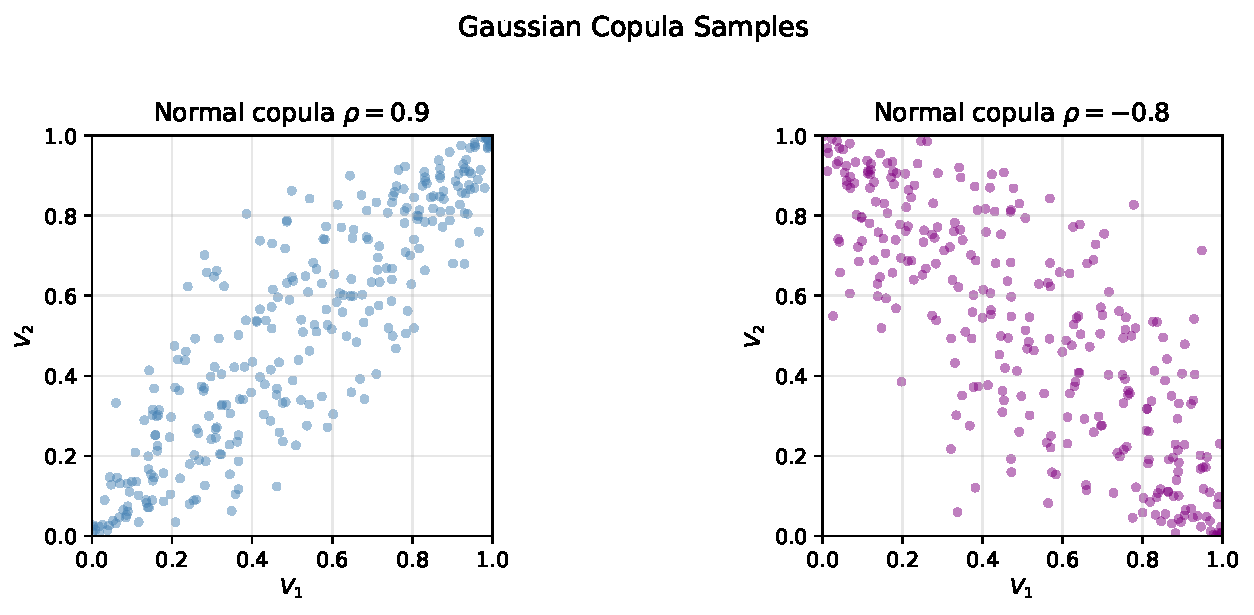
\includegraphics[width=0.65\textwidth]{fig_normal_copula}
    \caption{Gaussian copula: $\rho=0.9$ (left) and $\rho=-0.8$ (right).}
  \end{figure}

  \textbf{Using Copulas to Construct Joint Distributions (Example 3.9.10):}

  Given Exp(1) marginal for $X'$ and Par(1) for $Y'$:
  \begin{enumerate}
    \item Sample $(V_1,V_2)$ from a Gaussian copula with $\rho$.
    \item Transform: $X' = F_{\mathrm{Exp}}^{-1}(V_1) = -\log(1-V_1)$,
      $Y' = F_{\mathrm{Par}}^{-1}(V_2) = \frac{1}{1-V_2}-1$.
  \end{enumerate}
  This preserves the marginal distributions while changing the dependence structure.
\end{frame}

\begin{frame}[fragile]{3.9 Python: Gaussian Copula}
  \begin{lstlisting}[style=python, caption={Gaussian copula with specified marginals}]
import numpy as np
from scipy.stats import norm

rng = np.random.default_rng(42)

def sample_gaussian_copula(rho, n, rng):
    """Sample (V1, V2) from Gaussian copula with correlation rho."""
    Sigma = np.array([[1, rho], [rho, 1]])
    A = np.linalg.cholesky(Sigma)
    Z = rng.standard_normal((2, n))
    W = A @ Z
    return norm.cdf(W[0]), norm.cdf(W[1])

def to_exp_pareto(V1, V2):
    """Transform copula samples to Exp(1) x Pareto(1) marginals."""
    X = -np.log(1 - V1)           # F_Exp^{-1}(V1)
    Y = 1.0 / (1 - V2) - 1        # F_Par^{-1}(V2) for Par(alpha=1)
    return X, Y

V1, V2 = sample_gaussian_copula(rho=0.8, n=1000, rng=rng)
X, Y   = to_exp_pareto(V1, V2)
print(f"Corr(X,Y) = {np.corrcoef(X, Y)[0,1]:.3f}")
  \end{lstlisting}
\end{frame}

% ============================================================
\section{3.10 Heaviness of Distributions}
% ============================================================

\begin{frame}[allowframebreaks]{3.10 Can We See the Heaviness of a Distribution?}
  \textbf{Setting:} Compare i.i.d.\ sequences $X_1,X_2,\ldots$ with the same mean ($=1$)
  but different tails.  Look at:
  \begin{itemize}
    \item Running average $S_n/n = \frac{1}{n}\sum_{i=1}^n X_i$,
    \item Individual time series $(X_i)$.
  \end{itemize}

  \begin{columns}
    \column{0.48\textwidth}
    \begin{block}{Light vs Heavy Tails}
      \begin{tabular}{lll}
        \toprule
        Distribution & Mean & Tail \\
        \midrule
        $\NN(1,1)$ & 1 & Light \\
        $\mathrm{Exp}(1)$ & 1 & Light \\
        $\mathrm{LN}(-1/2,1)$ & 1 & Heavy \\
        $\mathrm{W}(1/2,\sqrt{2})$ & 1 & Heavy \\
        $0.2\cdot\mathrm{Par}(1.2)$ & 1 & Very heavy \\
        \bottomrule
      \end{tabular}
    \end{block}

    \column{0.50\textwidth}
    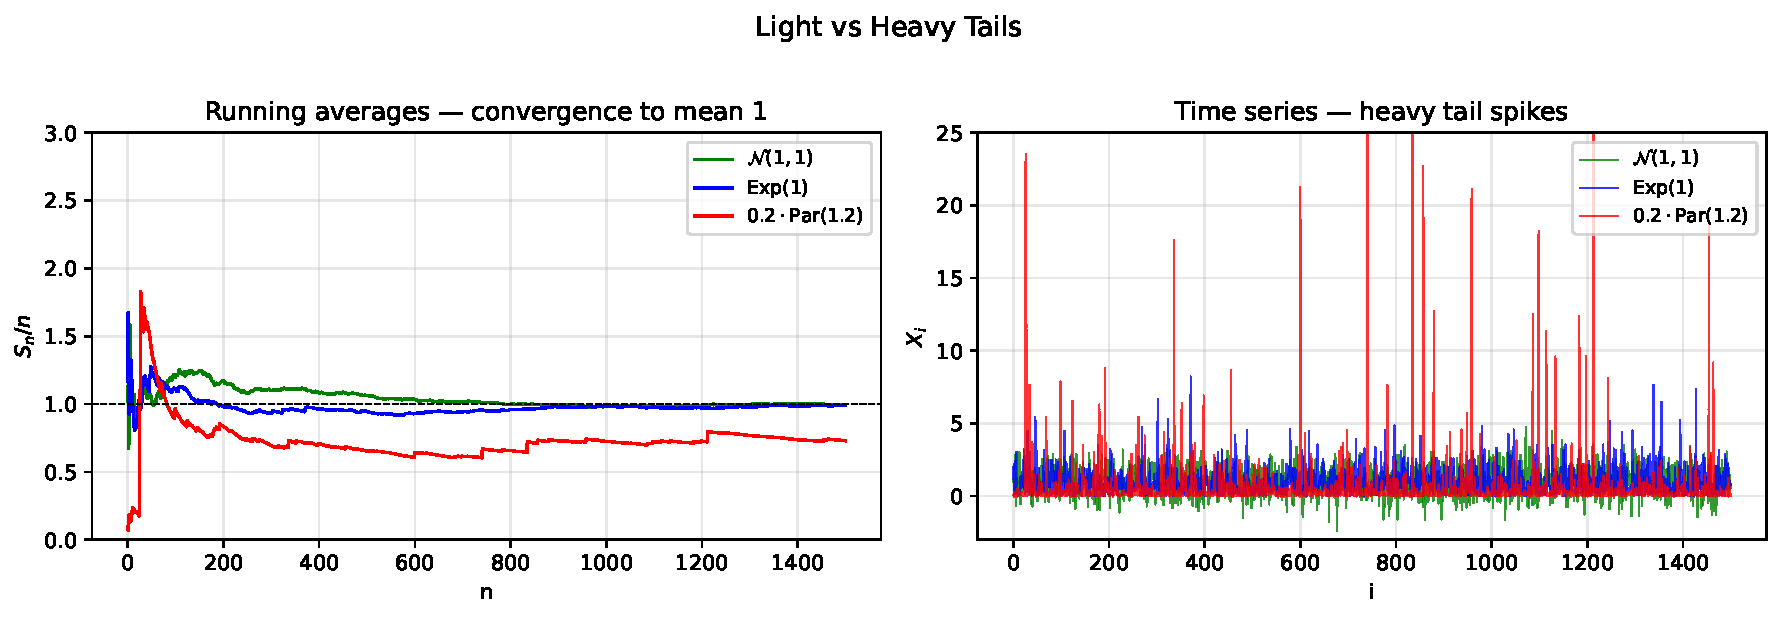
\includegraphics[width=\textwidth]{fig_heavy_tail}
  \end{columns}

  \framebreak

  \begin{block}{QQ Plots for Tail Detection}
    Plot the sample quantiles of $X$ against theoretical quantiles of $\NN(0,1)$:
    \begin{itemize}
      \item \textbf{Light-tailed:} points approximately on a straight line.
      \item \textbf{Heavy-tailed:} upper right (and lower left) bend upward.
      \item \textbf{Skewed:} asymmetric deviations.
    \end{itemize}
  \end{block}

  \begin{figure}
    \centering
    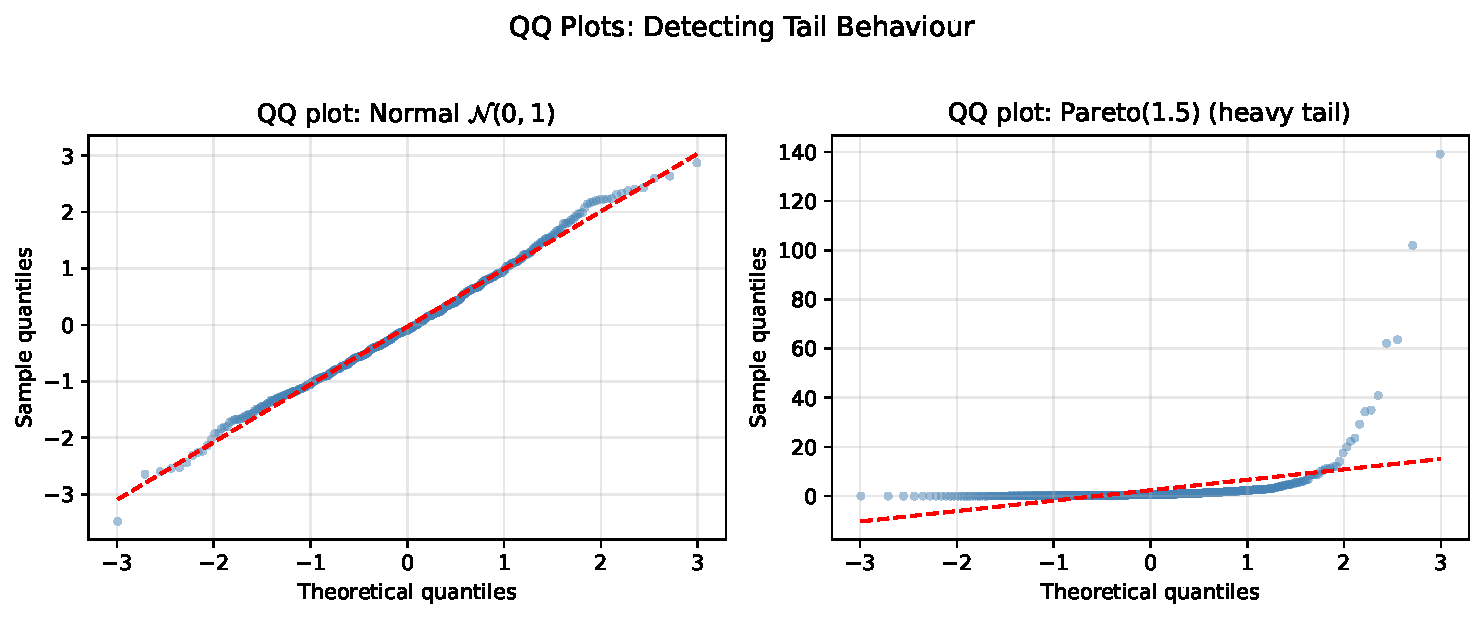
\includegraphics[width=0.70\textwidth]{fig_qq_plots}
    \caption{QQ plots: Normal (left, straight line) vs Pareto(1.5) (right, heavy-tail bend).}
  \end{figure}

  \textbf{Key observation:} The Pareto distribution has \emph{infinite variance}
  for $\alpha\le 2$; this makes $S_n/n$ converge extremely slowly, with large spikes.
\end{frame}

% ============================================================
\section{Summary}
% ============================================================

\begin{frame}[allowframebreaks]{Chapter 3 --- Summary of Methods}
  \begin{block}{Method Overview}
    \begin{tabular}{@{}lll@{}}
      \toprule
      Method & When to use & Key idea \\
      \midrule
      ITM (Alg.\ 6) & $F^{\leftarrow}$ available & $X = F^{\leftarrow}(U)$ \\
      ITM-d (Alg.\ 9) & Discrete, finite mean & Sequential accumulation \\
      ITR (Alg.\ 10) & $(a,b,0)$ class PMFs & Ratio recursion \\
      Geo.\ closed form & $\mathrm{Geo}(p)$ & $X=\lfloor\log U/\log p\rfloor$ \\
      DB (Alg.\ 11) & Binomial $B(n,p)$ & Sum of Bernoullis \\
      Erlang & $\mathrm{Erl}(n,\lambda)$ & Product of Uniforms \\
      DP (Alg.\ 12) & Poisson $\mathrm{Poi}(\lambda)$ & Renewal process \\
      AR-d (Alg.\ 14) & Discrete, $p_j\le cq_j$ & Accept with prob $p_j/(cq_j)$ \\
      AR-c (Alg.\ 16) & Continuous, $f\le cg$ & Geometric area under curve \\
      Composition & Mixture $f=\sum p_j g_j$ & Sample component, then value \\
      Box-Muller (Alg.\ 20) & Normal pairs & Polar transform \\
      Marsaglia-Bray (Alg.\ 21) & Normal pairs & Polar in 2D ball \\
      Cholesky & Multivariate normal & $\mathbf{X}=\mathbf{A}\mathbf{Z}+\boldsymbol{\mu}$ \\
      Normal trick & $\UU(S_{d-1})$ & Normalize $\NN(0,\mathbf{Id})$ \\
      Cond.\ ITM & Joint densities & Marginal then conditional \\
      Copula & Flexible dependence & Sklar's theorem \\
      \bottomrule
    \end{tabular}
  \end{block}

  \framebreak

  \begin{columns}
    \column{0.48\textwidth}
    \begin{block}{Key Formulas}
      \begin{align*}
        \text{ITM: } & X = F^{\leftarrow}(U) \\[4pt]
        \text{Exp: } & X = -\tfrac{1}{\lambda}\log U \\[4pt]
        \text{Pareto: } & X = U^{-1/\alpha} - 1 \\[4pt]
        \text{Geo: } & X = \lfloor \tfrac{\log U}{\log p}\rfloor \\[4pt]
        \text{Erlang: } & X = -\tfrac{\log(\prod U_i)}{\lambda} \\[4pt]
        \text{Box-Muller: }& Z = \sqrt{-2\log U_1}\cos(2\pi U_2) \\[4pt]
        \text{Multivariate: }& \mathbf{X} = \mathbf{A}\mathbf{Z}+\boldsymbol{\mu}
      \end{align*}
    \end{block}

    \column{0.50\textwidth}
    \begin{block}{Design Principles}
      \begin{itemize}
        \item AR method: choose $c = \sup f(x)/g(x)$ as small as possible.
        \item Efficiency $= 1/c$ (acceptance probability).
        \item Composition: excellent when $f$ is a finite mixture.
        \item Copulas: separate marginals from dependence structure (Sklar).
        \item Sphere sampling: normalize i.i.d.\ normals (exact, no rejection).
        \item QQ plots: visual tool to detect tail behaviour.
      \end{itemize}
    \end{block}
  \end{columns}
\end{frame}

% ============================================================
\section*{References}
% ============================================================

\begin{frame}{3.11 Bibliographical Notes}
  \begin{itemize}
    \item \textbf{Devroye (1986)} --- \textit{Non-Uniform Random Variate Generation}.
          Comprehensive reference for all methods in this chapter.
    \item \textbf{Knuth (1997)} --- \textit{The Art of Computer Programming, Vol.\ 2}.
          Classic treatment of the inverse transform method.
    \item \textbf{Asmussen \& Glynn (2007)} --- Fr?chet-Hoeffding bounds and copulas.
    \item \textbf{Box \& Muller (1958)} --- Original Box-Muller algorithm paper.
    \item \textbf{Marsaglia \& Bray (1964)} --- Polar method (Marsaglia-Bray).
    \item \textbf{Glasserman (2004)} --- ITM for normal r.v.s and Beasley-Springer-Moro.
    \item \textbf{Madras (2002)} --- AR-c for Gamma distribution.
    \item \textbf{Wichura (1988), AS241} --- Algorithm behind \texttt{scipy.stats.norm.ppf}.
    \item \textbf{Embrechts \& Hofert} --- Properties of copulas and generalized inverses.
    \item \textbf{Dagpunar (2007)} --- Composition method, Gamma sampling.
  \end{itemize}
\end{frame}

\end{document}
